\documentclass[a4paper,oneside]{report}
\usepackage{titlesec}
\usepackage[numbers,sort&compress]{natbib}
\usepackage[parfill]{parskip}
\usepackage{fancyhdr}
\usepackage{hyperref}
\usepackage{makecell}
\usepackage{graphicx}
\usepackage{multirow}

\setcounter{tocdepth}{4}
\setcounter{secnumdepth}{4}
\hypersetup{hidelinks}
\pagestyle{fancy}
\fancyhead[L,RO]{\leftmark\chaptertitlename}
\fancyhf{}
\cfoot{\thepage}

\titleformat{\chapter}{\normalfont\bfseries\huge}{\thechapter.}{20pt}{\huge}

\renewcommand{\headrulewidth}{0pt}
\renewcommand{\contentsname}{Table Of Contents}
\renewcommand{\bibname}{References}
\newenvironment{tableItem}{\begin{itemize}\setlength{\itemindent}{-6mm}}{\end{itemize}}

\begin{document}
	\begin{titlepage}
	\raggedleft
	
	\rule{1pt}{\textheight}
	\hspace{0.05\textwidth}
	\parbox[b]{0.75\textwidth}{
		
		{\Huge\bfseries Python Deployment Framework}\\[2\baselineskip]
		{\large\textit{CS4227 - Software Design and Architecture}}\\[4\baselineskip]
		{\Large\textsc{student name - student number}}\\[1\baselineskip]
		{\Large\textsc{student name - student number}}\\[1\baselineskip]
		{\Large\textsc{student name - student number}}\\[1\baselineskip]
		{\Large\textsc{student name - student number}}\\[1\baselineskip]
		{\Large\textsc{student name - student number}}\\[1\baselineskip]
		
		\vspace{0.25\textheight}
	}
\end{titlepage}
	\tableofcontents
	\begin{table}
\centering
\vspace*{-3cm}
\hspace*{-4cm}
\renewcommand{\arraystretch}{1.0}
\resizebox*{20cm}{27cm}{%
\begin{tabular}{|>{\centering}m{14.29mm}| >{\centering}m{14.29mm}| >{\centering}m{14.29mm}| >{\centering}m{14.29mm}| >{\centering}m{14.29mm}| >{\centering}m{14.29mm}| >{\centering}m{14.29mm}| >{\centering}m{14.29mm}| >{\centering}m{14.29mm}| >{\centering}m{14.29mm}| >{\centering}m{14.29mm}| >{\centering}m{14.29mm}| >{\centering}m{14.29mm}| >{\centering\arraybackslash}m{14.29mm}|}
	\hline
	\multicolumn{14}{|c|}{\textbf{CS4227: Software Design \& Architecture}} \\
	\multicolumn{14}{|c|}{\textbf{\underline{Guidance} on Marking Scheme for Team-Based Project:}} \\
	\multicolumn{14}{|c|}{\textbf{Semester 1, 2017-2018}} \\
	\multicolumn{14}{|c|}{(Version 2 18-09-2017)} \\
	\hline

	\multicolumn{7}{|l|}{Name 1: Jay Conroy} & \multicolumn{7}{l|}{ID1: 13148583} \\
	\multicolumn{7}{|l|}{Name 2: Russell Hickey} & \multicolumn{7}{l|}{ID1: 14141264} \\
	\multicolumn{7}{|l|}{Name 3: Oliver Gavin} & \multicolumn{7}{l|}{ID1: 14161044} \\
	\multicolumn{7}{|l|}{Name 4: Kevin O'Brien} & \multicolumn{7}{l|}{ID1: 14117428} \\
	\multicolumn{7}{|l|}{Name 5: Jonathan Lloyd} & \multicolumn{7}{l|}{ID1: 14117495} \\ \hline

	\multicolumn{1}{|c|}{} & \multicolumn{3}{c|}{\textbf{Item}} & \multicolumn{7}{c|}{\textbf{Detailed Description}} & \multicolumn{2}{c|}{
		\begin{tabular}{c|c}
			\multicolumn{2}{c}{\makecell{\textbf{Marks} \\ \textbf{Allocated}}} \\ \hline
			Sub- & Total
		\end{tabular}
	} & \makecell{\textbf{Marks} \\ \textbf{Awarded}} \\ \hline

	\multicolumn{1}{|c|}{\multirow{5}{*}{1-2}} & \multicolumn{3}{c|}{\multirow{5}{*}{Presentation}} & \multicolumn{7}{p{0.5\textwidth}|}{
		\begin{list}{\labelitemi}{\leftmargin=3mm}
			\item General Presentation
			\item Adherence to guidelines - cover sheet, blank marking scheme, table of contents
		\end{list}
	} & \multirow{5}{*}{} & \multirow{5}{*}{2} & \\ \hline

	\multicolumn{1}{|c|}{\multirow{6}{*}{3}} & \multicolumn{3}{c|}{\multirow{6}{*}{Requirements}} & \multicolumn{7}{p{0.5\textwidth}|}{
		\begin{list}{\labelitemi}{\leftmargin=3mm}
			\item Narrative, Use Case diagram, and SAMPLE Use Case Description
			\item Discussion on NFRs with a focus on architectural use cases (quality attributes)
		\end{list}
	} & \multirow{6}{*}{\makecell{1\\\\2}} & \multirow{6}{*}{3} & \\ \hline

	\multicolumn{1}{|c|}{\multirow{6}{*}{4}} & \multicolumn{3}{c|}{\multirow{6}{*}{\makecell{Discussion on \\Architectural and \\Design Patterns}}} & \multicolumn{7}{p{0.5\textwidth}|}{
		\begin{list}{\labelitemi}{\leftmargin=3mm}
			\item The Interceptor architectural pattern
			\item Discussion of 6 patterns
			\item One must be selected through independent research
		\end{list}
	} & \multirow{6}{*}{\makecell{1\\2\\1}} & \multirow{6}{*}{4} & \\ \hline

	\multicolumn{1}{|c|}{5} & \multicolumn{3}{c|}{\makecell{System \\ Architecture}} & \multicolumn{7}{p{0.5\textwidth}|}{} & & 4 & \\ \hline

	\multicolumn{1}{|c|}{\multirow{4}{*}{6}} & \multicolumn{3}{c|}{\multirow{4}{*}{\makecell{Structural and \\Behavioural \\Diagram}}} & \multicolumn{7}{p{0.5\textwidth}|}{
		Class and interaction diagram with
		\begin{list}{\labelitemi}{\leftmargin=3mm}
			\item Correct application of design patterns
			\item All patterns integrated
		\end{list}
	} & \multirow{4}{*}{\makecell{2\\1\\1}} & \multirow{4}{*}{4} & \\ \hline

	\multicolumn{1}{|c|}{\multirow{11}{*}{7}} & \multicolumn{3}{c|}{\multirow{11}{*}{Code}} & \multicolumn{7}{p{0.5\textwidth}|}{
		\begin{list}{\labelitemi}{\leftmargin=3mm}
			\item Matches/Supports/Realises diagrams
			\item Interceptor pattern correctly implemented
			\item Design Patterns correctly implemented
			\item Exposes intent, supporting documentation, naming conventions clearly identify design patterns used

			\item At least 4 packages, one developed by each team member
		\end{list}
	} & \multirow{11}{*}{\makecell{\\3\\3\\\\6\\\\3\\\\\\P/F}} & \multirow{11}{*}{15} & \\ \hline

	\multicolumn{1}{|c|}{8} & \multicolumn{3}{c|}{Added Value} & \multicolumn{7}{p{0.5\textwidth}|}{Two examples, 3 marks each} & & 6 & \\ \hline

	\multicolumn{1}{|c|}{\multirow{5}{*}{9}} & \multicolumn{3}{c|}{\multirow{5}{*}{Testing}} & \multicolumn{7}{p{0.5\textwidth}|}{
		\begin{list}{\labelitemi}{\leftmargin=3mm}
			\item Design of test cases
			\item Automated
			\item Analysis of results
		\end{list}
	} & \multirow{5}{*}{\makecell{1\\1\\1}} & \multirow{5}{*}{3} & \\ \hline

	\multicolumn{1}{|c|}{\multirow{2}{*}{10}} & \multicolumn{3}{c|}{\multirow{2}{*}{Issues}} & \multicolumn{7}{p{0.5\textwidth}|}{\makecell{Satisfactorily documented.\\No marks awarded}
	} &  & \multirow{2}{*}{N/A} & \\ \hline

	\multicolumn{1}{|c|}{\multirow{4}{*}{11}} & \multicolumn{3}{c|}{\multirow{4}{*}{\makecell{Evaluation /\\Critique}}} & \multicolumn{7}{p{0.5\textwidth}|}{Is it the case that the patterns selected supported relevant architectural use cases? If not, why not? Any alternatives?} & & \multirow{4}{*}{3} & \\ \hline

	\multicolumn{1}{|c|}{12} & \multicolumn{3}{c|}{References} & \multicolumn{7}{p{0.5\textwidth}|}{} & & 1 & \\ \hline

	\multicolumn{1}{|c|}{} & \multicolumn{3}{c|}{\multirow{3}{*}{Interview}} & \multicolumn{7}{p{0.5\textwidth}|}{
		\begin{list}{\labelitemi}{\leftmargin=3mm}
			\item Competent code inspection
			\item Working demo
		\end{list}
	} & & \multirow{3}{*}{P/F} & \\ \hline

	\multicolumn{12}{|c|}{\textbf{SUB-TOTAL(A)}} & 45 & \\ \hline

\end{tabular}}
\end{table}


	\chapter{Requirements}


\section{Scenario}
TODO

\section{Use Cases and Use Case Descriptions}
  \subsection{Use Case Diagram}
    \begin{figure}[H]
        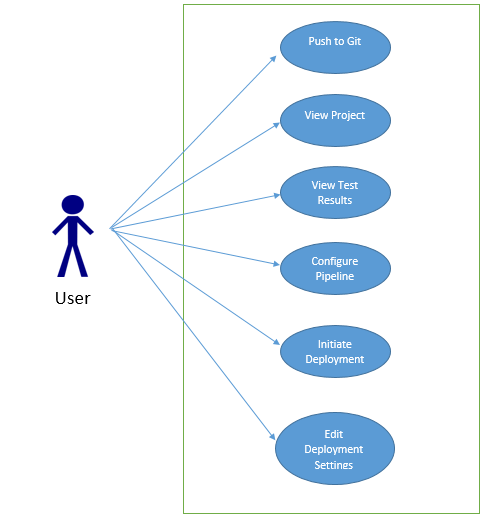
\includegraphics[width = 1.2\linewidth]{diagrams/UseCaseDiagram}
        \caption{Use Case Diagram}
        \label{fig:use_case_diagram}
      \end{figure}
      
   \subsection{Use Case Description}
   \begin{figure}[H]
       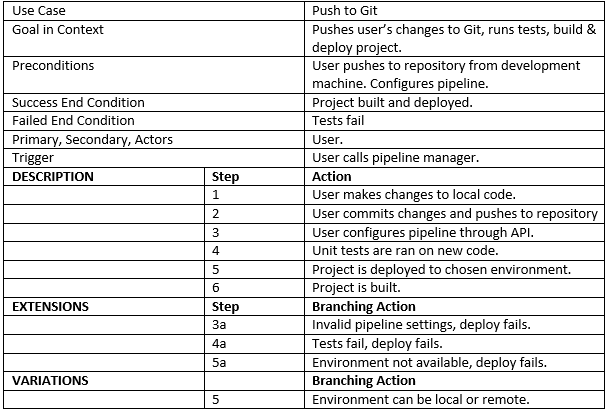
\includegraphics[width = 1.2\linewidth]{diagrams/DetailedUseCase}
       \caption{Use Case Description}
       \label{fig:use_case_description}
     \end{figure}    


\section{Architectural Use Cases}
TODO

\subsubsection{Tactics?}
TODO


\section{Non-Functional Requirements}

In software systems, non-functional requirements (NFRs) describe how a system works, while functional requirements describe what the system should do. Unlike functional requirements, NFRs are not captured in use cases and cannot be analysed by drawing sequence diagrams or state charts. Non-functional requirements can be subjective and can be evaluated differently by different people. For these reasons, NFRs can be difficult to deal with. Yet, dealing with NFRs can be vital for the success of a software system. \cite{nfrs} Failing to meet a non-functional requirement can result in systems that fail to satisfy business and user needs or can result in unfulfilled mandatory requirements imposed by regulatory or standards agencies. NFRs usually cannot be implemented in a single module of the system and can be categorised into 3 main types according to Gorton (2006) \cite{sw-arch}:
\begin{itemize}
  \item Quality attributes / architectural use cases e.g. ``ilities"
  \item Business e.g. FDA standard compliant
  \item Technical e.g. must develop in Python and use Flask microframework
\end{itemize}

\subsection{Security}
Software security protects systems from unintended and unauthorized access and protects against malicious attacks and other risks, so that the software can continue to function correctly under such potential risks. Encryption is the most effective way to achieve data security. During user authentication, the user's credentials (username and password) should be encrypted so that they can be transferred over the framework securely. The encrypted values can then be compared with encrypted information in the database.

Audit logs should be verbose enough to support forensics. All account modification events as well as any system warnings or errors should be logged and monitored. This can be supported using the Interceptor design pattern. An example event log after a system modification would include information such as date, time, user, action, entity changed, prior value and new value. Web-based issue trackers could also provide a way for users of the framework to report bugs and vulnerabilities. Such reported vulnerabilities should only be accessible by individuals with prior permission from the security team.

\subsection{Extensibility}
Good architectural design is supported by system components that can be extended easily by both the developer of the framework to create new versions of the components and by third-parties (users) that have to adapt components for use in specific software systems. Good extensibility in a software system can be achieved by architectural design patterns such as the Abstract Factory and the Interceptor. Using an object-orientated language such as Python helps with the implementation of design patterns. The deployment framework being developed will most likely feature glass-box extensibility. This refers to a software system that may be extended with third party extensions that are separate from the original framework in a way that does not affect the original framework. The clean separation of the framework and the third-parties' extensions makes it easier to understand and maintain extensions. \cite{glassbox}

\subsection{Performance}
Performance is a measure of the amount of work accomplished by a computer system. High performance involves a system having short response times, low utilisation of computing resources (compute, storage, networking), high availability and short data transmission time. Performance can be improved by distributing work across multiple machines in the system. Types of work that could be distributed for a deployment framework include builds/testing, deployments and database utilisation across disks (NoSQL databases give up some features of the traditional databases for speed and more importantly for horizontal scaling).

\subsection{Configuration Management}
Configuration management is the task of tracking and controlling changes in a system. If a failure occurs in a system due to an incorrect configuration, configuration files can determine what was changed and who changed it. Distributing text files containing configuration information is a common way to manage configurations in a software system. Master copies of important configuration files are kept in a central location and distributed to machines that require them. Centralization enables version control, reducing the time taken to make changes across large groups of hosts. Using a simple version control system such as Git will ensure any config changes are logged and can be audited if the need arises.

Ansible and Chef are examples of configuration management tools. Both tools achieve similiar results but work in different ways. Chef operates on a client-server model, where a Chef server stores configuration files called Cookbooks. The client nodes run the Chef client software, which performs the automation and config management upon receiving instructions from the Chef server. On the other hand, Ansible is agentless, requiring nothing on target hosts systems other than SSH and Python. This makes Ansible easy to work with and has excellent inbuilt security with SSH.

	\chapter{Design Patterns}

\section{Creational}
Creational design patterns are design patterns that deal with object creation
mechanisms, trying to create objects in a manner suitable to the situation. The basic form of object
creation could result in design problems or added complexity to the design. Creational design patterns
solve this problem by controlling this object creation.

\subsection{Abstract Factory}
The Abstract Factory design pattern adds another layer of abstraction to the Factory design pattern.
The Abstract Factory provides us with a framework that allows us to create families of related or
dependent objects without specifying their concrete classes. So at runtime, the abstract factory is
coupled with any desired factory which can create objects of desired type.

\section{Structural}
Structural design patterns are design patterns that ease the design by identifying a simple way to
realize relationships between entities.

\subsection{Bridge}
The Bridge design pattern allows us to separate the abstraction from the implementation, thus
allowing us to hide the implementation from the client and only providing the abstraction.
Use when:
\begin{itemize}
	\item we want run-time binding of the implementation
	\item we have a collection of related classes resulting from a coupled interface and numerous
	      implementations
	\item we want to share an implementation among multiple objects
	\item we need to map orthogonal class hierarchies
\end{itemize}

\subsection{Composite}
The composite pattern is used to group objects into tree structures to represent whole-part hierachies. This pattern lets clients treat individual objects and compositions of objects uniformly. \cite{sourcemaking}

\section{Behavioral}
In software engineering, behavioral design patterns are design patterns that identify common communication patterns between objects and realize these patterns. By doing so, these patterns increase flexibility in carrying out this communication. \cite{sourcemaking}

\subsection{Memento}
The memento pattern allows us to capture and externalise an objects state so that the object can be returned to this state later on.
Steps:
\begin{itemize}
	\item Ask originator to create and return a memento.
	\item Save the memento.
	\item Update the state of the originator.
	\item Retrieve a memento from storage.
	\item Ask originator to recreate its previous state using this memento.
\end{itemize}

\subsection{State}
The state pattern allows an object to change it's behaviour when it changes it's internal state. The main object is called the context and this is the object that keeps the state. When the state needs to be changed we ca

\subsection{Visitor}
The visitors purpose is to abstract functionality that can be applied to an aggregate hierarchy of \'Element\' objects. \cite{sourcemaking} This allows the operations to be put into their own class which stops polluting the objects class.
\begin{itemize}
	\item The visitor asks the element to accept it's visit.
	\item The element accepts and passes itself to the visitors visit method.
\end{itemize}

	\chapter{Architecture}
% TODO make diagrams more readable, discussion?

  The framework has been implemented as a 3-tier architecture. This allowed us to easily
  separate responsibilities and minimise coupling. The architecture focuses on allowing
  third party integrations easily with the use of the interceptor architectural pattern.
  To make it easy for clients to use the framework, a server is supplied which exposes
  a REST API. A pluggable adapter is used in order to allow the integration of other
  database systems which is an important feature.

  \section{Architectural Diagram}
  Clients can integrate on two levels. Clients can attach to dispatcher directly themselves or
  clients can register their modules. The framework then runs a flask REST server.
  A user can assemble their own pipeline via REST or a GUI. The framework in in charge or creating
  the supplied interceptors and attaching them to dispatchers and managing a pipeline on a thread.

  \section{Package Diagram}
    \begin{figure}[H]
        \hspace{-8em}
        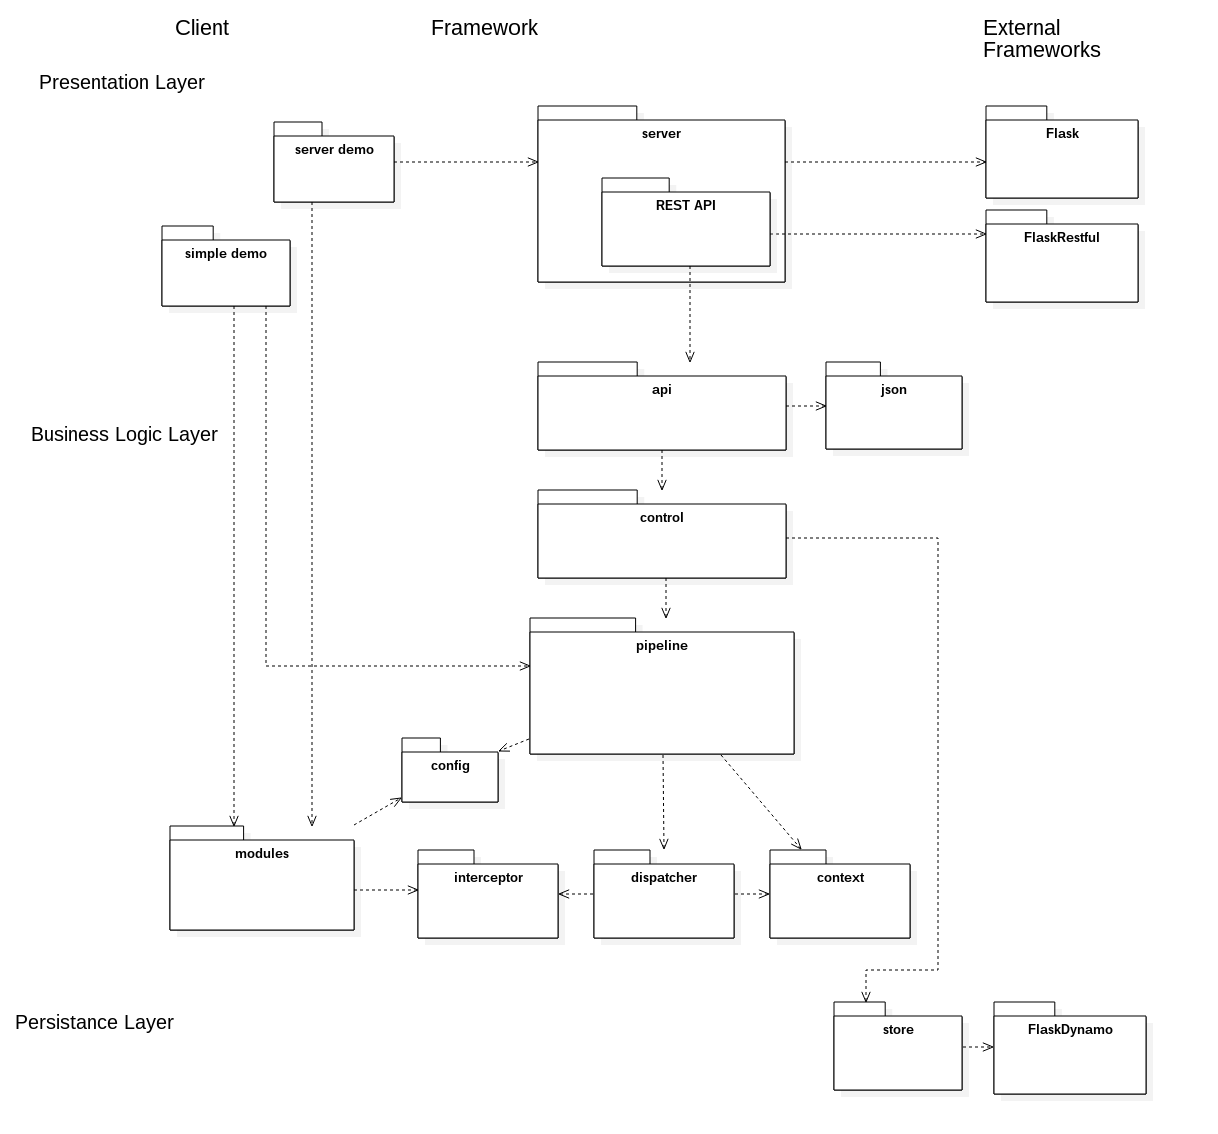
\includegraphics[width = 1.5\linewidth]{diagrams/architecture.png}
        \caption{Package Diagram}
        \label{fig:architecture_packages}
      \end{figure}

  \section{Class Diagram}
    \begin{figure}[H]
        \hspace{-4em}
        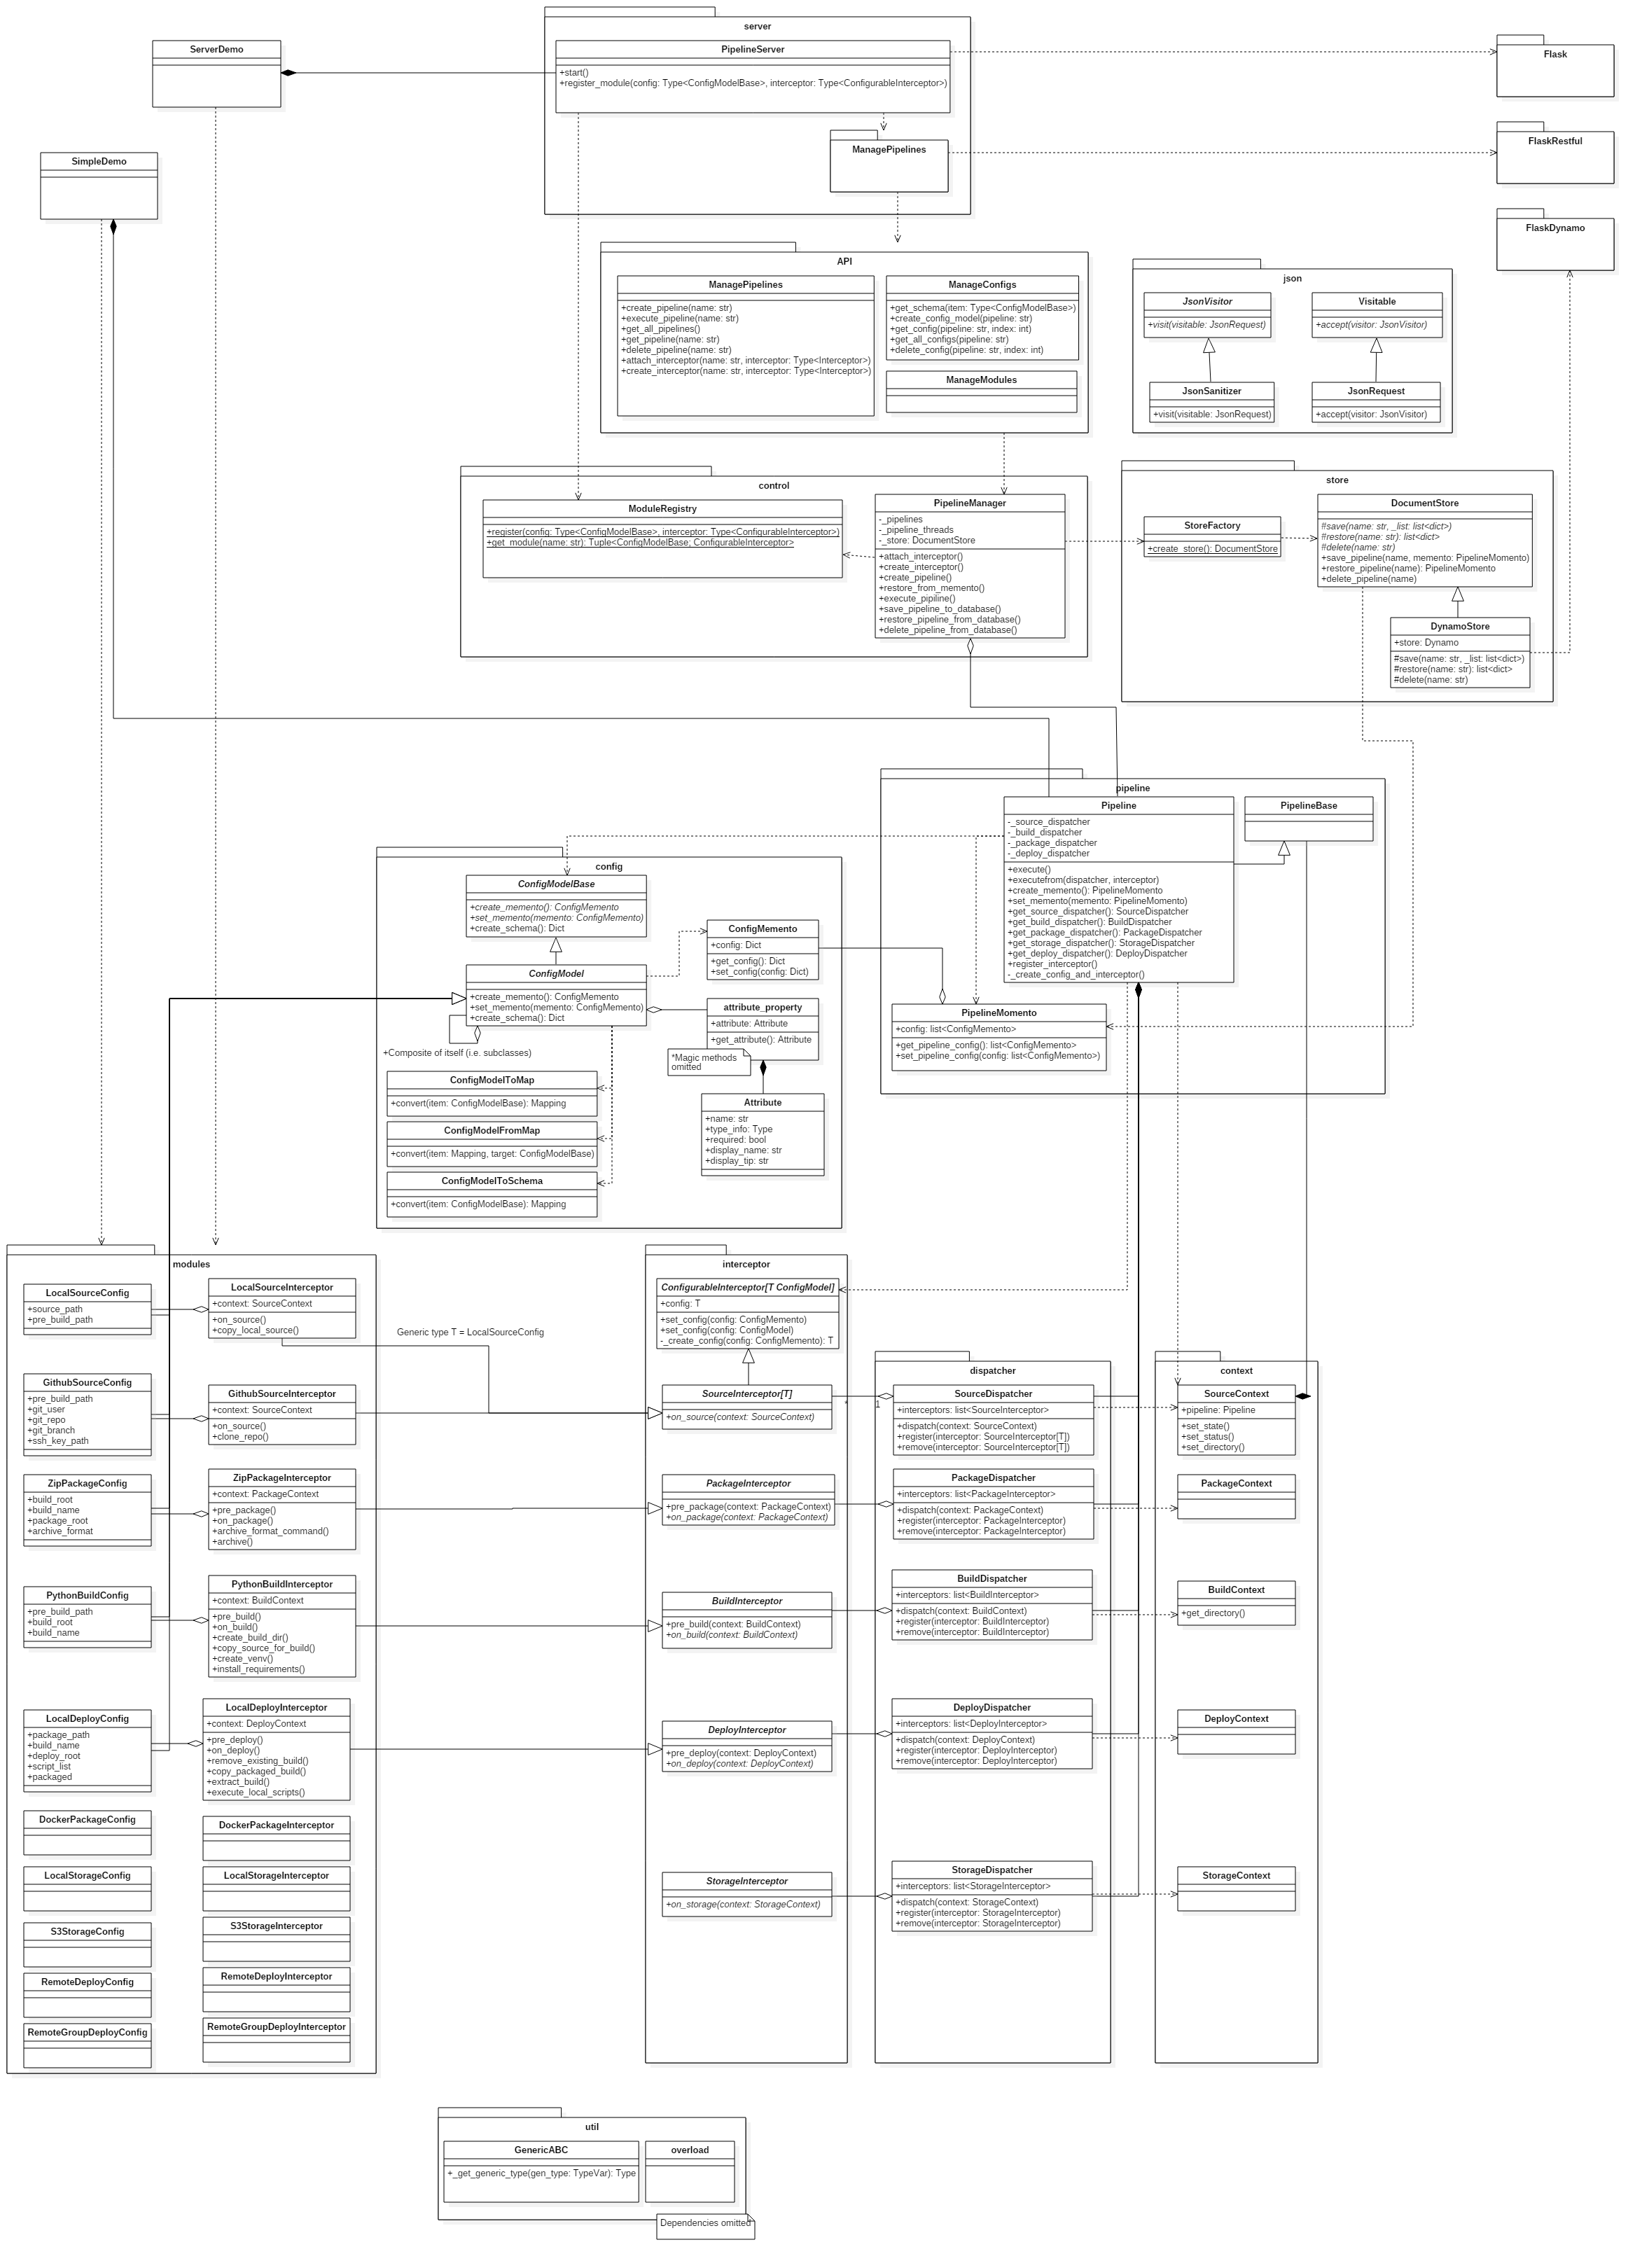
\includegraphics[width = 1.2\linewidth]{diagrams/architecture_classes.png}
        \caption{Architecture Class Diagram}
        \label{fig:architecture_classes}
      \end{figure}

    \section{Class Diagram Fragments}
    TODO


   \section{Sequence Diagram}
	   \begin{figure}[H]
	   	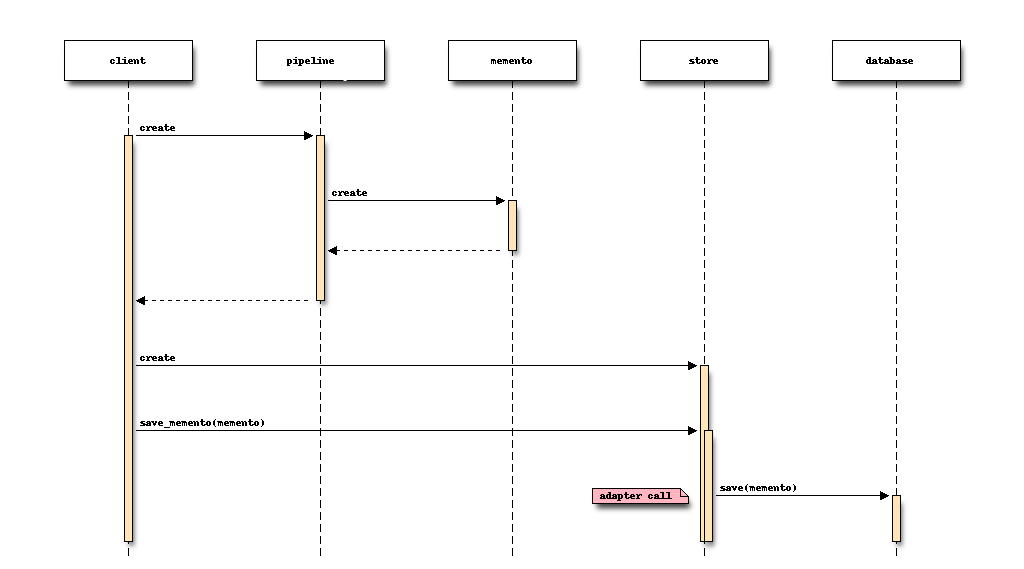
\includegraphics[width = 1.2\linewidth]{diagrams/sequence_diagram.png}
	   	\caption{Pluggable Adapter Sequence Diagram}
	   \end{figure}

TODO structural diagram




	\bibliographystyle{unsrtnat}
	\bibliography{references}
\end{document}
